% Options for packages loaded elsewhere
\PassOptionsToPackage{unicode}{hyperref}
\PassOptionsToPackage{hyphens}{url}
%
\documentclass[
]{article}
\usepackage{amsmath,amssymb}
\usepackage{iftex}
\ifPDFTeX
  \usepackage[T1]{fontenc}
  \usepackage[utf8]{inputenc}
  \usepackage{textcomp} % provide euro and other symbols
\else % if luatex or xetex
  \usepackage{unicode-math} % this also loads fontspec
  \defaultfontfeatures{Scale=MatchLowercase}
  \defaultfontfeatures[\rmfamily]{Ligatures=TeX,Scale=1}
\fi
\usepackage{lmodern}
\ifPDFTeX\else
  % xetex/luatex font selection
\fi
% Use upquote if available, for straight quotes in verbatim environments
\IfFileExists{upquote.sty}{\usepackage{upquote}}{}
\IfFileExists{microtype.sty}{% use microtype if available
  \usepackage[]{microtype}
  \UseMicrotypeSet[protrusion]{basicmath} % disable protrusion for tt fonts
}{}
\makeatletter
\@ifundefined{KOMAClassName}{% if non-KOMA class
  \IfFileExists{parskip.sty}{%
    \usepackage{parskip}
  }{% else
    \setlength{\parindent}{0pt}
    \setlength{\parskip}{6pt plus 2pt minus 1pt}}
}{% if KOMA class
  \KOMAoptions{parskip=half}}
\makeatother
\usepackage{xcolor}
\usepackage[margin=1in]{geometry}
\usepackage{color}
\usepackage{fancyvrb}
\newcommand{\VerbBar}{|}
\newcommand{\VERB}{\Verb[commandchars=\\\{\}]}
\DefineVerbatimEnvironment{Highlighting}{Verbatim}{commandchars=\\\{\}}
% Add ',fontsize=\small' for more characters per line
\usepackage{framed}
\definecolor{shadecolor}{RGB}{248,248,248}
\newenvironment{Shaded}{\begin{snugshade}}{\end{snugshade}}
\newcommand{\AlertTok}[1]{\textcolor[rgb]{0.94,0.16,0.16}{#1}}
\newcommand{\AnnotationTok}[1]{\textcolor[rgb]{0.56,0.35,0.01}{\textbf{\textit{#1}}}}
\newcommand{\AttributeTok}[1]{\textcolor[rgb]{0.13,0.29,0.53}{#1}}
\newcommand{\BaseNTok}[1]{\textcolor[rgb]{0.00,0.00,0.81}{#1}}
\newcommand{\BuiltInTok}[1]{#1}
\newcommand{\CharTok}[1]{\textcolor[rgb]{0.31,0.60,0.02}{#1}}
\newcommand{\CommentTok}[1]{\textcolor[rgb]{0.56,0.35,0.01}{\textit{#1}}}
\newcommand{\CommentVarTok}[1]{\textcolor[rgb]{0.56,0.35,0.01}{\textbf{\textit{#1}}}}
\newcommand{\ConstantTok}[1]{\textcolor[rgb]{0.56,0.35,0.01}{#1}}
\newcommand{\ControlFlowTok}[1]{\textcolor[rgb]{0.13,0.29,0.53}{\textbf{#1}}}
\newcommand{\DataTypeTok}[1]{\textcolor[rgb]{0.13,0.29,0.53}{#1}}
\newcommand{\DecValTok}[1]{\textcolor[rgb]{0.00,0.00,0.81}{#1}}
\newcommand{\DocumentationTok}[1]{\textcolor[rgb]{0.56,0.35,0.01}{\textbf{\textit{#1}}}}
\newcommand{\ErrorTok}[1]{\textcolor[rgb]{0.64,0.00,0.00}{\textbf{#1}}}
\newcommand{\ExtensionTok}[1]{#1}
\newcommand{\FloatTok}[1]{\textcolor[rgb]{0.00,0.00,0.81}{#1}}
\newcommand{\FunctionTok}[1]{\textcolor[rgb]{0.13,0.29,0.53}{\textbf{#1}}}
\newcommand{\ImportTok}[1]{#1}
\newcommand{\InformationTok}[1]{\textcolor[rgb]{0.56,0.35,0.01}{\textbf{\textit{#1}}}}
\newcommand{\KeywordTok}[1]{\textcolor[rgb]{0.13,0.29,0.53}{\textbf{#1}}}
\newcommand{\NormalTok}[1]{#1}
\newcommand{\OperatorTok}[1]{\textcolor[rgb]{0.81,0.36,0.00}{\textbf{#1}}}
\newcommand{\OtherTok}[1]{\textcolor[rgb]{0.56,0.35,0.01}{#1}}
\newcommand{\PreprocessorTok}[1]{\textcolor[rgb]{0.56,0.35,0.01}{\textit{#1}}}
\newcommand{\RegionMarkerTok}[1]{#1}
\newcommand{\SpecialCharTok}[1]{\textcolor[rgb]{0.81,0.36,0.00}{\textbf{#1}}}
\newcommand{\SpecialStringTok}[1]{\textcolor[rgb]{0.31,0.60,0.02}{#1}}
\newcommand{\StringTok}[1]{\textcolor[rgb]{0.31,0.60,0.02}{#1}}
\newcommand{\VariableTok}[1]{\textcolor[rgb]{0.00,0.00,0.00}{#1}}
\newcommand{\VerbatimStringTok}[1]{\textcolor[rgb]{0.31,0.60,0.02}{#1}}
\newcommand{\WarningTok}[1]{\textcolor[rgb]{0.56,0.35,0.01}{\textbf{\textit{#1}}}}
\usepackage{graphicx}
\makeatletter
\def\maxwidth{\ifdim\Gin@nat@width>\linewidth\linewidth\else\Gin@nat@width\fi}
\def\maxheight{\ifdim\Gin@nat@height>\textheight\textheight\else\Gin@nat@height\fi}
\makeatother
% Scale images if necessary, so that they will not overflow the page
% margins by default, and it is still possible to overwrite the defaults
% using explicit options in \includegraphics[width, height, ...]{}
\setkeys{Gin}{width=\maxwidth,height=\maxheight,keepaspectratio}
% Set default figure placement to htbp
\makeatletter
\def\fps@figure{htbp}
\makeatother
\setlength{\emergencystretch}{3em} % prevent overfull lines
\providecommand{\tightlist}{%
  \setlength{\itemsep}{0pt}\setlength{\parskip}{0pt}}
\setcounter{secnumdepth}{-\maxdimen} % remove section numbering
\ifLuaTeX
  \usepackage{selnolig}  % disable illegal ligatures
\fi
\IfFileExists{bookmark.sty}{\usepackage{bookmark}}{\usepackage{hyperref}}
\IfFileExists{xurl.sty}{\usepackage{xurl}}{} % add URL line breaks if available
\urlstyle{same}
\hypersetup{
  pdftitle={Intro\_R\_Spatial\_Tools},
  pdfauthor={RMM},
  hidelinks,
  pdfcreator={LaTeX via pandoc}}

\title{Intro\_R\_Spatial\_Tools}
\author{RMM}
\date{2023-09-22}

\begin{document}
\maketitle

\hypertarget{r-markdown}{%
\subsubsection{R Markdown}\label{r-markdown}}

Both R and Python have libraries that can process files referred to as
``shape files''. Details on the definition and development of the format
can be read at {[}wikipedia{]}
(\url{https://en.wikipedia.org/wiki/Shapefile}). An important thing to
know is that whereas shape file refers to data that is used to represent
geographical features, it needs 3 files to be operational.

\hypertarget{shp}{%
\subsubsection{.shp}\label{shp}}

where coordinates of geographical features are kept.

\hypertarget{shx}{%
\subsubsection{.shx}\label{shx}}

an indexing file for geometric features.

\hypertarget{dbf}{%
\subsubsection{.dbf}\label{dbf}}

data that is associated with the geometric features. The folder we are
going to download exists within the US Census Bureau website. From the
website we navigate to where the
\href{https://www2.census.gov/geo/tiger/TIGER2021/COUNTY/}{shape files
for all the counties in USA are located}

As you can see from the download, there are additional files present
besides the .shp, .shx and .dbf. These are files that are not required
for R and Python to create informative maps but we will keep them in our
folder. In this project we make use of a multitude of spatial tools and
functions for statistical analysis but for now we will focus only on the
mapping aspects and the simple features,
\href{https://r-spatial.github.io/sf/}{sf package}.

\begin{Shaded}
\begin{Highlighting}[]
\CommentTok{\# Loading the library, if you are using Windows you will have to make sure you have Rtools before being able to use the library {-}{-}\textgreater{}}
\FunctionTok{library}\NormalTok{(sf)}
\end{Highlighting}
\end{Shaded}

\begin{verbatim}
## Linking to GEOS 3.11.2, GDAL 3.6.2, PROJ 9.2.0; sf_use_s2() is TRUE
\end{verbatim}

\begin{Shaded}
\begin{Highlighting}[]
\CommentTok{\#We downloaded the shape zip folder, unzipped all the files in it to the data folder and read it in with the read\_sf command{-}{-}\textgreater{} }
\NormalTok{shape }\OtherTok{\textless{}{-}} \FunctionTok{read\_sf}\NormalTok{(}\AttributeTok{dsn =} \StringTok{"C:/Users/rm84/Desktop/research/HMM/data/tl\_2021\_us\_county.shp"}\NormalTok{)}
\CommentTok{\#as can be seen from the dim command you have 3234 observations (counties) and 18 features associated with each county}
\FunctionTok{dim}\NormalTok{(shape)}
\end{Highlighting}
\end{Shaded}

\begin{verbatim}
## [1] 3234   18
\end{verbatim}

\begin{Shaded}
\begin{Highlighting}[]
\CommentTok{\#In R, objects have attributes. The shape object has 5 of these}
\FunctionTok{length}\NormalTok{(}\FunctionTok{attributes}\NormalTok{(shape))}
\end{Highlighting}
\end{Shaded}

\begin{verbatim}
## [1] 5
\end{verbatim}

\begin{Shaded}
\begin{Highlighting}[]
\CommentTok{\#We will look at only the first attribute\textquotesingle{}s values}
\FunctionTok{attributes}\NormalTok{(shape)[}\DecValTok{1}\NormalTok{]}
\end{Highlighting}
\end{Shaded}

\begin{verbatim}
## $names
##  [1] "STATEFP"  "COUNTYFP" "COUNTYNS" "GEOID"    "NAME"     "NAMELSAD"
##  [7] "LSAD"     "CLASSFP"  "MTFCC"    "CSAFP"    "CBSAFP"   "METDIVFP"
## [13] "FUNCSTAT" "ALAND"    "AWATER"   "INTPTLAT" "INTPTLON" "geometry"
\end{verbatim}

\begin{Shaded}
\begin{Highlighting}[]
\CommentTok{\#Names function will give us the values in the first attribute }
\FunctionTok{names}\NormalTok{(shape)}
\end{Highlighting}
\end{Shaded}

\begin{verbatim}
##  [1] "STATEFP"  "COUNTYFP" "COUNTYNS" "GEOID"    "NAME"     "NAMELSAD"
##  [7] "LSAD"     "CLASSFP"  "MTFCC"    "CSAFP"    "CBSAFP"   "METDIVFP"
## [13] "FUNCSTAT" "ALAND"    "AWATER"   "INTPTLAT" "INTPTLON" "geometry"
\end{verbatim}

\begin{Shaded}
\begin{Highlighting}[]
\CommentTok{\#We will be working with only the Californian state }
\CommentTok{\#selecting California via FIPS state code as you can see selection is done via base R via the \%in\% statement}
\NormalTok{shape}\OtherTok{=}\NormalTok{shape[(shape}\SpecialCharTok{$}\NormalTok{STATEFP }\SpecialCharTok{\%in\%} \StringTok{\textquotesingle{}06\textquotesingle{}}\NormalTok{),]}

\CommentTok{\#We could look at a very simple set of plots}
\FunctionTok{plot}\NormalTok{(shape)}
\end{Highlighting}
\end{Shaded}

\begin{verbatim}
## Warning: plotting the first 9 out of 17 attributes; use max.plot = 17 to plot
## all
\end{verbatim}

\includegraphics{index_files/figure-latex/unnamed-chunk-1-1.pdf}

\begin{Shaded}
\begin{Highlighting}[]
\CommentTok{\#The shape function has 17 attributes and R chooses to plot a smaller number of them to fit the screen. }


\CommentTok{\#We would rather do something a bit more useful and plot one of the attributes we are interested in}
\FunctionTok{plot}\NormalTok{(shape[}\DecValTok{15}\NormalTok{])}
\end{Highlighting}
\end{Shaded}

\includegraphics{index_files/figure-latex/unnamed-chunk-1-2.pdf}

\begin{Shaded}
\begin{Highlighting}[]
\CommentTok{\#Note that if you wrote plot(shape$AWATER) you get a scatterplot.}
\end{Highlighting}
\end{Shaded}

A good \href{https://r-spatial.github.io/sf/articles/}{vignette} exists
to explain the sf package.

Before we introduce better looking plots we need to understand how to
merge data to a shapefile.

We created a dataframe named \bold{CASummary} by wrangling through a
multitude of datasets which will be discussed on a later post. It is
important to look at some of the output from this dataset.

\begin{Shaded}
\begin{Highlighting}[]
\FunctionTok{library}\NormalTok{(sf)}
\FunctionTok{library}\NormalTok{(ggplot2)}
\FunctionTok{library}\NormalTok{(ggspatial)}
\FunctionTok{library}\NormalTok{(ggpubr)}
\FunctionTok{library}\NormalTok{(cowplot)}
\end{Highlighting}
\end{Shaded}

\begin{verbatim}
## 
## Attaching package: 'cowplot'
\end{verbatim}

\begin{verbatim}
## The following object is masked from 'package:ggpubr':
## 
##     get_legend
\end{verbatim}

\begin{Shaded}
\begin{Highlighting}[]
\FunctionTok{library}\NormalTok{(viridis)}
\end{Highlighting}
\end{Shaded}

\begin{verbatim}
## Loading required package: viridisLite
\end{verbatim}

\begin{Shaded}
\begin{Highlighting}[]
\NormalTok{data\_for\_spatial}\OtherTok{=}\FunctionTok{read.table}\NormalTok{(}\AttributeTok{header=}\ConstantTok{TRUE}\NormalTok{,}\AttributeTok{sep=}\StringTok{\textquotesingle{},\textquotesingle{}}\NormalTok{,}\StringTok{\textquotesingle{}C:/Users/rm84/Documents/data\_for\_spatial.csv\textquotesingle{}}\NormalTok{)}
\NormalTok{poverty\_for\_spatial}\OtherTok{=}\FunctionTok{read.table}\NormalTok{(}\AttributeTok{header=}\ConstantTok{TRUE}\NormalTok{,}\AttributeTok{sep=}\StringTok{\textquotesingle{},\textquotesingle{}}\NormalTok{,}\StringTok{\textquotesingle{}C:/Users/rm84/Documents/poverty\_for\_spatial.csv\textquotesingle{}}\NormalTok{)}
\CommentTok{\#Each of the 58 counties of California in alphabetical and FIPS order have 164 columns of information associated with it. The last 154 columns represent 2 sets of variables across a 77 biweek time period. Mortality and Vaccinations Rates.}
\FunctionTok{dim}\NormalTok{(data\_for\_spatial)}
\end{Highlighting}
\end{Shaded}

\begin{verbatim}
## [1]  58 244
\end{verbatim}

\begin{Shaded}
\begin{Highlighting}[]
\CommentTok{\#First 10 values in the data.frame object}
\CommentTok{\#}
\FunctionTok{names}\NormalTok{(data\_for\_spatial)[}\DecValTok{1}\SpecialCharTok{:}\DecValTok{10}\NormalTok{]}
\end{Highlighting}
\end{Shaded}

\begin{verbatim}
##  [1] "X"         "ID"        "Counties"  "Poverty20" "Poverty21" "Income20" 
##  [7] "Income21"  "Density"   "Gini20"    "Gini21"
\end{verbatim}

\begin{Shaded}
\begin{Highlighting}[]
\CommentTok{\#identify the unique keys in each object. shape and \#CASUmmary has 58 unique GEOID and ID values representing \#the counties in California They are 3 digit FIPS codes.}
\CommentTok{\#001 003 etc...}
\CommentTok{\#it is important to first write the shape file.}
\NormalTok{shapeanddata}\OtherTok{=}\FunctionTok{merge}\NormalTok{(shape,data\_for\_spatial,}\AttributeTok{by.y=}\StringTok{"ID"}\NormalTok{,}\AttributeTok{by.x=}\StringTok{"COUNTYFP"}\NormalTok{)}
\NormalTok{meanpov}\OtherTok{=}\FunctionTok{mean}\NormalTok{(poverty\_for\_spatial[,}\DecValTok{4}\NormalTok{])}
\end{Highlighting}
\end{Shaded}

\begin{verbatim}
## Warning in mean.default(poverty_for_spatial[, 4]): argument is not numeric or
## logical: returning NA
\end{verbatim}

\begin{Shaded}
\begin{Highlighting}[]
\NormalTok{sdpov}\OtherTok{=}\FunctionTok{sd}\NormalTok{(poverty\_for\_spatial[,}\DecValTok{4}\NormalTok{])}
\end{Highlighting}
\end{Shaded}

\begin{verbatim}
## Warning in var(if (is.vector(x) || is.factor(x)) x else as.double(x), na.rm =
## na.rm): NAs introduced by coercion
\end{verbatim}

\begin{Shaded}
\begin{Highlighting}[]
\CommentTok{\#\_spatial options require ggspatial package}
\CommentTok{\#operations on data are allowed. In this instance we used it}
\CommentTok{\#to unnormalize the poverty variable}
\NormalTok{map\_Pov20}\OtherTok{=}\FunctionTok{ggplot}\NormalTok{() }\SpecialCharTok{+}
  \FunctionTok{annotation\_spatial}\NormalTok{(shapeanddata) }\SpecialCharTok{+}
  \FunctionTok{layer\_spatial}\NormalTok{(shapeanddata, }\FunctionTok{aes}\NormalTok{(}\AttributeTok{fill =}\NormalTok{ (Poverty20}\SpecialCharTok{*}\NormalTok{sdpov}\SpecialCharTok{+}\NormalTok{meanpov)))}\SpecialCharTok{+}
  \FunctionTok{labs}\NormalTok{(}\AttributeTok{fill =} \StringTok{"Pov. 20"}\NormalTok{)}

\NormalTok{map\_Pov20}
\end{Highlighting}
\end{Shaded}

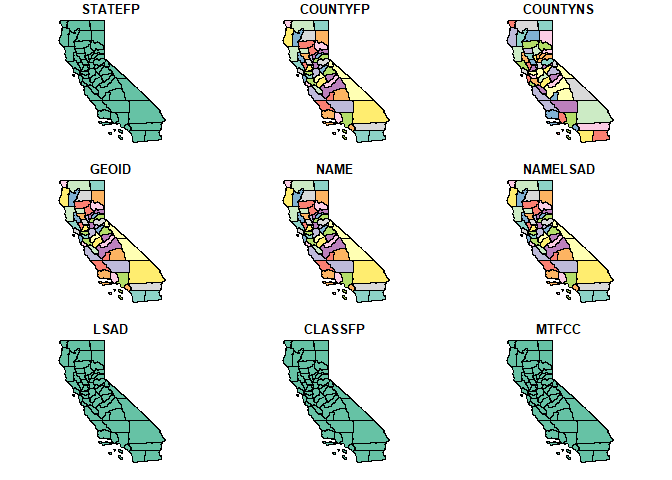
\includegraphics{index_files/figure-latex/unnamed-chunk-2-1.pdf}

\begin{Shaded}
\begin{Highlighting}[]
\NormalTok{map\_Pov21}\OtherTok{=}\FunctionTok{ggplot}\NormalTok{() }\SpecialCharTok{+}
  \FunctionTok{annotation\_spatial}\NormalTok{(shapeanddata) }\SpecialCharTok{+}
  \FunctionTok{layer\_spatial}\NormalTok{(shapeanddata, }\FunctionTok{aes}\NormalTok{(}\AttributeTok{fill =}\NormalTok{ (Poverty21}\SpecialCharTok{*}\NormalTok{sdpov}\SpecialCharTok{+}\NormalTok{meanpov)))}\SpecialCharTok{+}
  \FunctionTok{labs}\NormalTok{(}\AttributeTok{fill =} \StringTok{"Pov. 21"}\NormalTok{)}

\CommentTok{\#Different scales we need to put them on the same scale}
\FunctionTok{plot\_grid}\NormalTok{(map\_Pov20,map\_Pov21)}
\end{Highlighting}
\end{Shaded}

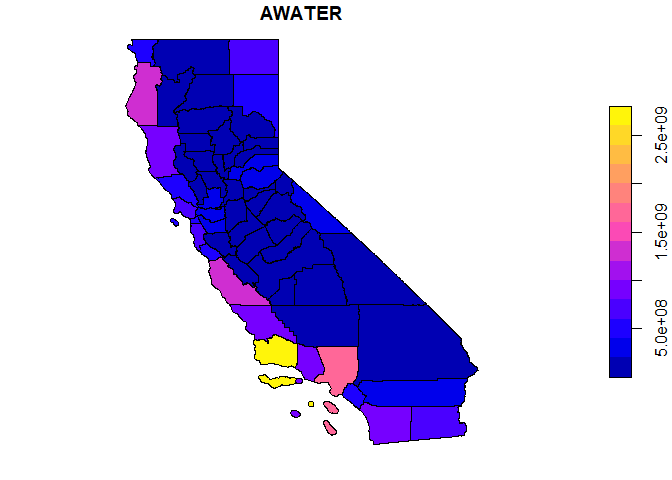
\includegraphics{index_files/figure-latex/unnamed-chunk-2-2.pdf}

\begin{Shaded}
\begin{Highlighting}[]
\DocumentationTok{\#\#\#\#\#\#\#\#\#\#\#\#\#\#\#\#\#\#\#\#\#\#\#\#\#\#\#\#\#\#\#\#\#\#\#\#\#\#\#\#\#}
\CommentTok{\#Let us hide the legend and use a common scale for these two years}
\NormalTok{map\_Pov20}\OtherTok{=}\FunctionTok{ggplot}\NormalTok{() }\SpecialCharTok{+}
  \FunctionTok{annotation\_spatial}\NormalTok{(shapeanddata) }\SpecialCharTok{+}
  \FunctionTok{layer\_spatial}\NormalTok{(shapeanddata, }\FunctionTok{aes}\NormalTok{(}\AttributeTok{fill =}\NormalTok{ (Poverty20}\SpecialCharTok{*}\NormalTok{sdpov}\SpecialCharTok{+}\NormalTok{meanpov)))}\SpecialCharTok{+}
  \FunctionTok{labs}\NormalTok{(}\AttributeTok{fill =} \StringTok{"Pov. 20"}\NormalTok{)}\SpecialCharTok{+}\FunctionTok{scale\_fill\_viridis}\NormalTok{(}\AttributeTok{limits =} \FunctionTok{c}\NormalTok{(}\DecValTok{0}\NormalTok{,}\DecValTok{22}\NormalTok{),}\AttributeTok{direction=}\SpecialCharTok{{-}}\DecValTok{1}\NormalTok{)}\SpecialCharTok{+}
  \FunctionTok{theme}\NormalTok{(}\AttributeTok{legend.position =} \StringTok{"none"}\NormalTok{,}\AttributeTok{plot.title =}\FunctionTok{element\_blank}\NormalTok{())}


\NormalTok{map\_Pov21}\OtherTok{=}\FunctionTok{ggplot}\NormalTok{() }\SpecialCharTok{+}
  \FunctionTok{annotation\_spatial}\NormalTok{(shapeanddata) }\SpecialCharTok{+}
  \FunctionTok{layer\_spatial}\NormalTok{(shapeanddata, }\FunctionTok{aes}\NormalTok{(}\AttributeTok{fill =}\NormalTok{ (Poverty21}\SpecialCharTok{*}\NormalTok{sdpov}\SpecialCharTok{+}\NormalTok{meanpov)))}\SpecialCharTok{+}
  \FunctionTok{labs}\NormalTok{(}\AttributeTok{fill =} \StringTok{"Pov. 21"}\NormalTok{)}\SpecialCharTok{+}\FunctionTok{scale\_fill\_viridis}\NormalTok{(}\AttributeTok{limits =} \FunctionTok{c}\NormalTok{(}\DecValTok{0}\NormalTok{,}\DecValTok{22}\NormalTok{),}\AttributeTok{direction=}\SpecialCharTok{{-}}\DecValTok{1}\NormalTok{)}

\CommentTok{\#This has obvious scale on the output issues }
\FunctionTok{plot\_grid}\NormalTok{(map\_Pov20,map\_Pov21)}
\end{Highlighting}
\end{Shaded}

\includegraphics{index_files/figure-latex/unnamed-chunk-2-3.pdf}

\begin{Shaded}
\begin{Highlighting}[]
\NormalTok{map\_Pov20}\OtherTok{=}\FunctionTok{ggplot}\NormalTok{() }\SpecialCharTok{+}
  \FunctionTok{annotation\_spatial}\NormalTok{(shapeanddata) }\SpecialCharTok{+}
  \FunctionTok{layer\_spatial}\NormalTok{(shapeanddata, }\FunctionTok{aes}\NormalTok{(}\AttributeTok{fill =}\NormalTok{ (Poverty20}\SpecialCharTok{*}\NormalTok{sdpov}\SpecialCharTok{+}\NormalTok{meanpov)))}\SpecialCharTok{+}
  \FunctionTok{theme}\NormalTok{(}\AttributeTok{legend.title=} \FunctionTok{element\_blank}\NormalTok{())}\SpecialCharTok{+}
  \FunctionTok{labs}\NormalTok{(}\AttributeTok{fill =} \StringTok{"Pov. 20"}\NormalTok{)}\SpecialCharTok{+}\FunctionTok{scale\_fill\_viridis}\NormalTok{(}\AttributeTok{limits =} \FunctionTok{c}\NormalTok{(}\DecValTok{0}\NormalTok{,}\DecValTok{22}\NormalTok{),}\AttributeTok{direction=}\SpecialCharTok{{-}}\DecValTok{1}\NormalTok{)}
  


\NormalTok{map\_Pov21}\OtherTok{=}\FunctionTok{ggplot}\NormalTok{() }\SpecialCharTok{+}
  \FunctionTok{annotation\_spatial}\NormalTok{(shapeanddata) }\SpecialCharTok{+}
  \FunctionTok{layer\_spatial}\NormalTok{(shapeanddata, }\FunctionTok{aes}\NormalTok{(}\AttributeTok{fill =}\NormalTok{ (Poverty21}\SpecialCharTok{*}\NormalTok{sdpov}\SpecialCharTok{+}\NormalTok{meanpov)))}\SpecialCharTok{+}\FunctionTok{annotate}\NormalTok{(}\StringTok{"text"}\NormalTok{, }\AttributeTok{x =} \SpecialCharTok{{-}}\DecValTok{118}\NormalTok{, }\AttributeTok{y =}\DecValTok{40}\NormalTok{ , }\AttributeTok{label =} \StringTok{"Merced"}\NormalTok{)}\SpecialCharTok{+}
  \FunctionTok{annotate}\NormalTok{(}\StringTok{"segment"}\NormalTok{, }\AttributeTok{color=}\StringTok{"red"}\NormalTok{, }\AttributeTok{x=}\SpecialCharTok{{-}}\DecValTok{118}\NormalTok{, }\AttributeTok{xend =} \SpecialCharTok{{-}}\FloatTok{120.5}\NormalTok{, }
           \AttributeTok{y=}\FloatTok{39.8}\NormalTok{, }
           \AttributeTok{yend=}\FloatTok{37.2}\NormalTok{, }\AttributeTok{arrow=}\FunctionTok{arrow}\NormalTok{(}\AttributeTok{length=}\FunctionTok{unit}\NormalTok{(}\FloatTok{0.2}\NormalTok{,}\StringTok{"cm"}\NormalTok{)))}\SpecialCharTok{+}
  \FunctionTok{labs}\NormalTok{(}\AttributeTok{fill =} \StringTok{"Pov. 21"}\NormalTok{)}\SpecialCharTok{+}\FunctionTok{scale\_fill\_viridis}\NormalTok{(}\AttributeTok{limits =} \FunctionTok{c}\NormalTok{(}\DecValTok{0}\NormalTok{,}\DecValTok{22}\NormalTok{),}\AttributeTok{direction=}\SpecialCharTok{{-}}\DecValTok{1}\NormalTok{)}



\NormalTok{map\_Pov2021 }\OtherTok{\textless{}{-}} \FunctionTok{ggarrange}\NormalTok{(}\AttributeTok{labels=}\FunctionTok{c}\NormalTok{(}\StringTok{"Poverty 2020"}\NormalTok{,}\StringTok{"Poverty 2021"}\NormalTok{),map\_Pov20, map\_Pov21, }\AttributeTok{nrow =} \DecValTok{1}\NormalTok{, }\AttributeTok{align =} \StringTok{"h"}\NormalTok{, }\AttributeTok{common.legend =} \ConstantTok{TRUE}\NormalTok{)}
\FunctionTok{annotate\_figure}\NormalTok{(}\AttributeTok{fig.lab.face=}\StringTok{"bold"}\NormalTok{,}\AttributeTok{fig.lab.size=}\DecValTok{14}\NormalTok{,}\AttributeTok{fig.lab.pos=}\StringTok{"top.left"}\NormalTok{,map\_Pov2021, }\AttributeTok{fig.lab =} \StringTok{"Maps of Poverty Percentages"}\NormalTok{)}
\end{Highlighting}
\end{Shaded}

\includegraphics{index_files/figure-latex/unnamed-chunk-2-4.pdf}

\end{document}
